\documentclass[12pt, twoside]{article}
% \documentclass[12pt, twoside]{article}
\usepackage[letterpaper, margin=1in, headsep=0.2in]{geometry}
\setlength{\headheight}{0.6in}
%\usepackage[english]{babel}
\usepackage[utf8]{inputenc}
\usepackage{microtype}
\usepackage{amsmath}
\usepackage{amssymb}
%\usepackage{amsfonts}
\usepackage[nomessages]{fp} %\FPeval{\var-name}{2*sin(pi/6)}
\usepackage{siunitx} %units in math. eg 20\milli\meter
\usepackage{yhmath} % for arcs, overparenth command
\usepackage{tikz} %graphics
\usetikzlibrary{quotes, angles, arrows, arrows.meta}
\usepackage{graphicx} %consider setting \graphicspath{{images/}}
\usepackage{parskip} %no paragraph indent
\usepackage{enumitem}
\usepackage{multicol}
\usepackage{venndiagram}

\usepackage{fancyhdr}
\pagestyle{fancy}
\fancyhf{}
\renewcommand{\headrulewidth}{0pt} % disable the underline of the header
\raggedbottom
\hfuzz=2mm %suppresses overfull box warnings

\usepackage{hyperref}
\usepackage{float}

\fancyhead[LE]{\thepage}
\fancyhead[RO]{\thepage \\ First and last name: \hspace{2.5cm} \,\\ Section: \hspace{2.5cm} \,}
\fancyhead[LO]{BECA/Huson/Geometry: Solid geometry \\* 7 March 2025}

\begin{document}
\subsubsection*{5.16 Test \hfill G.SRT.5 Use similarity criteria for triangles to solve problems}
\begin{enumerate}[itemsep=0.5cm]

\item A dilation maps $\triangle ABC \rightarrow \triangle ADE$. Given $AB=12$, $AC=15$, $BC=9$, $CE=20$. 
\begin{multicols}{2}
    Find the scale factor and side lengths:\\[0.5cm]
    $k=$\\[1cm]
    $DE=$\\[1cm]
    $AD=$\\[1cm]
    $BD=$\\
    \begin{flushright}
    \begin{tikzpicture}[scale=1.]
        \draw [thick]
        (0,0)node[below]{$A$}--
        (0:6)node[below]{$D$}--
        (30:8)node[above]{$E$}--cycle;
        \draw [thick]
        (0:3)node[below]{$B$}--
        (30:4)node[above left]{$C$};
        \node at (0:1.5)[below]{$12$};
        \node at (15:3.3)[right]{$9$};
        \node at (36:5.5)[right]{$20$};
        \node at (35:1.7)[above]{$15$};
    \end{tikzpicture}
    \end{flushright}
\end{multicols}

\subsubsection*{G.SRT.C.8 Use trigonometry to solve problems with right triangles}
\item As shown, right $\triangle ABC$ has $AC=5, BC=12, AB=13$, m$\angle C=90^\circ$. \\[0.25cm] 
Express each trigonometric ratio as a fraction.
  \begin{multicols}{2}
    \begin{enumerate}
      \item $\sin A =$
      \item $\cos A =$
      \item $\tan A =$ 
      \item Find the angle measure of $\angle A$ rounded to the \emph{nearest whole degree}. \vspace{1cm}
    \end{enumerate}
    \begin{center}
      \begin{tikzpicture}[scale=0.3]
        \draw [thick](0,0) node[below]{$A$}--
        (4,0) node[below]{$C$}--
        (4,9.5) node[right]{$B$}--cycle;
        \node at (2,-1){$5$};
        \node at (4,4)[right]{$12$};
        \node at (0.8,4.7){$13$};
        \draw (4,0)++(-0.6,0)--++(0,0.6)--+(0.6,0);
        \draw (0.75,0) arc [start angle=0, end angle=63, radius=0.75];
      \end{tikzpicture}
    \end{center}
  \end{multicols}\vspace{0.25cm}

\item At an angle of elevation of $15^\circ$, the top of a structure $B$ is visible from point $A$ on the ground 50 meters away, as shown below.

  Find the height $h$ of the structure to the \emph{nearest tenth of a meter}. \hfill (not to scale)
    \begin{flushright}
      \begin{tikzpicture}[scale=0.3]
        %\draw [-, thick] (0,0)--(35:23);
        \draw [-, thick] (-4,0)--
        (0,0)--
          (17,0)--
          (22,0)--
          (22,10)--(17,10)--(17,0);
        \draw [fill] (0,0) circle [radius=0.1] node[above left]{$A$};
        \draw [fill] (17,10) circle [radius=0.1] node[above right]{$B$};
        \draw [dashed] (0,0)--(17,10);
        \node at (3.8, 0)[above]{$15^\circ$};
        \node at (11, 0)[below]{50 m};
        \node at (17, 5)[right]{$h$};
      \end{tikzpicture}
      \end{flushright}




\end{enumerate}
\end{document}